% Use XeLaTeX / LuaLaTeX with a Chinese-capable document class.
% Preamble: \usepackage{graphicx}, \usepackage{subcaption}, \usepackage{placeins}
% Put the two PNG files alongside the main .tex, or set \graphicspath.
\begin{figure}[htbp]
  \centering
  \begin{subfigure}[t]{0.48\textwidth}
    \centering
    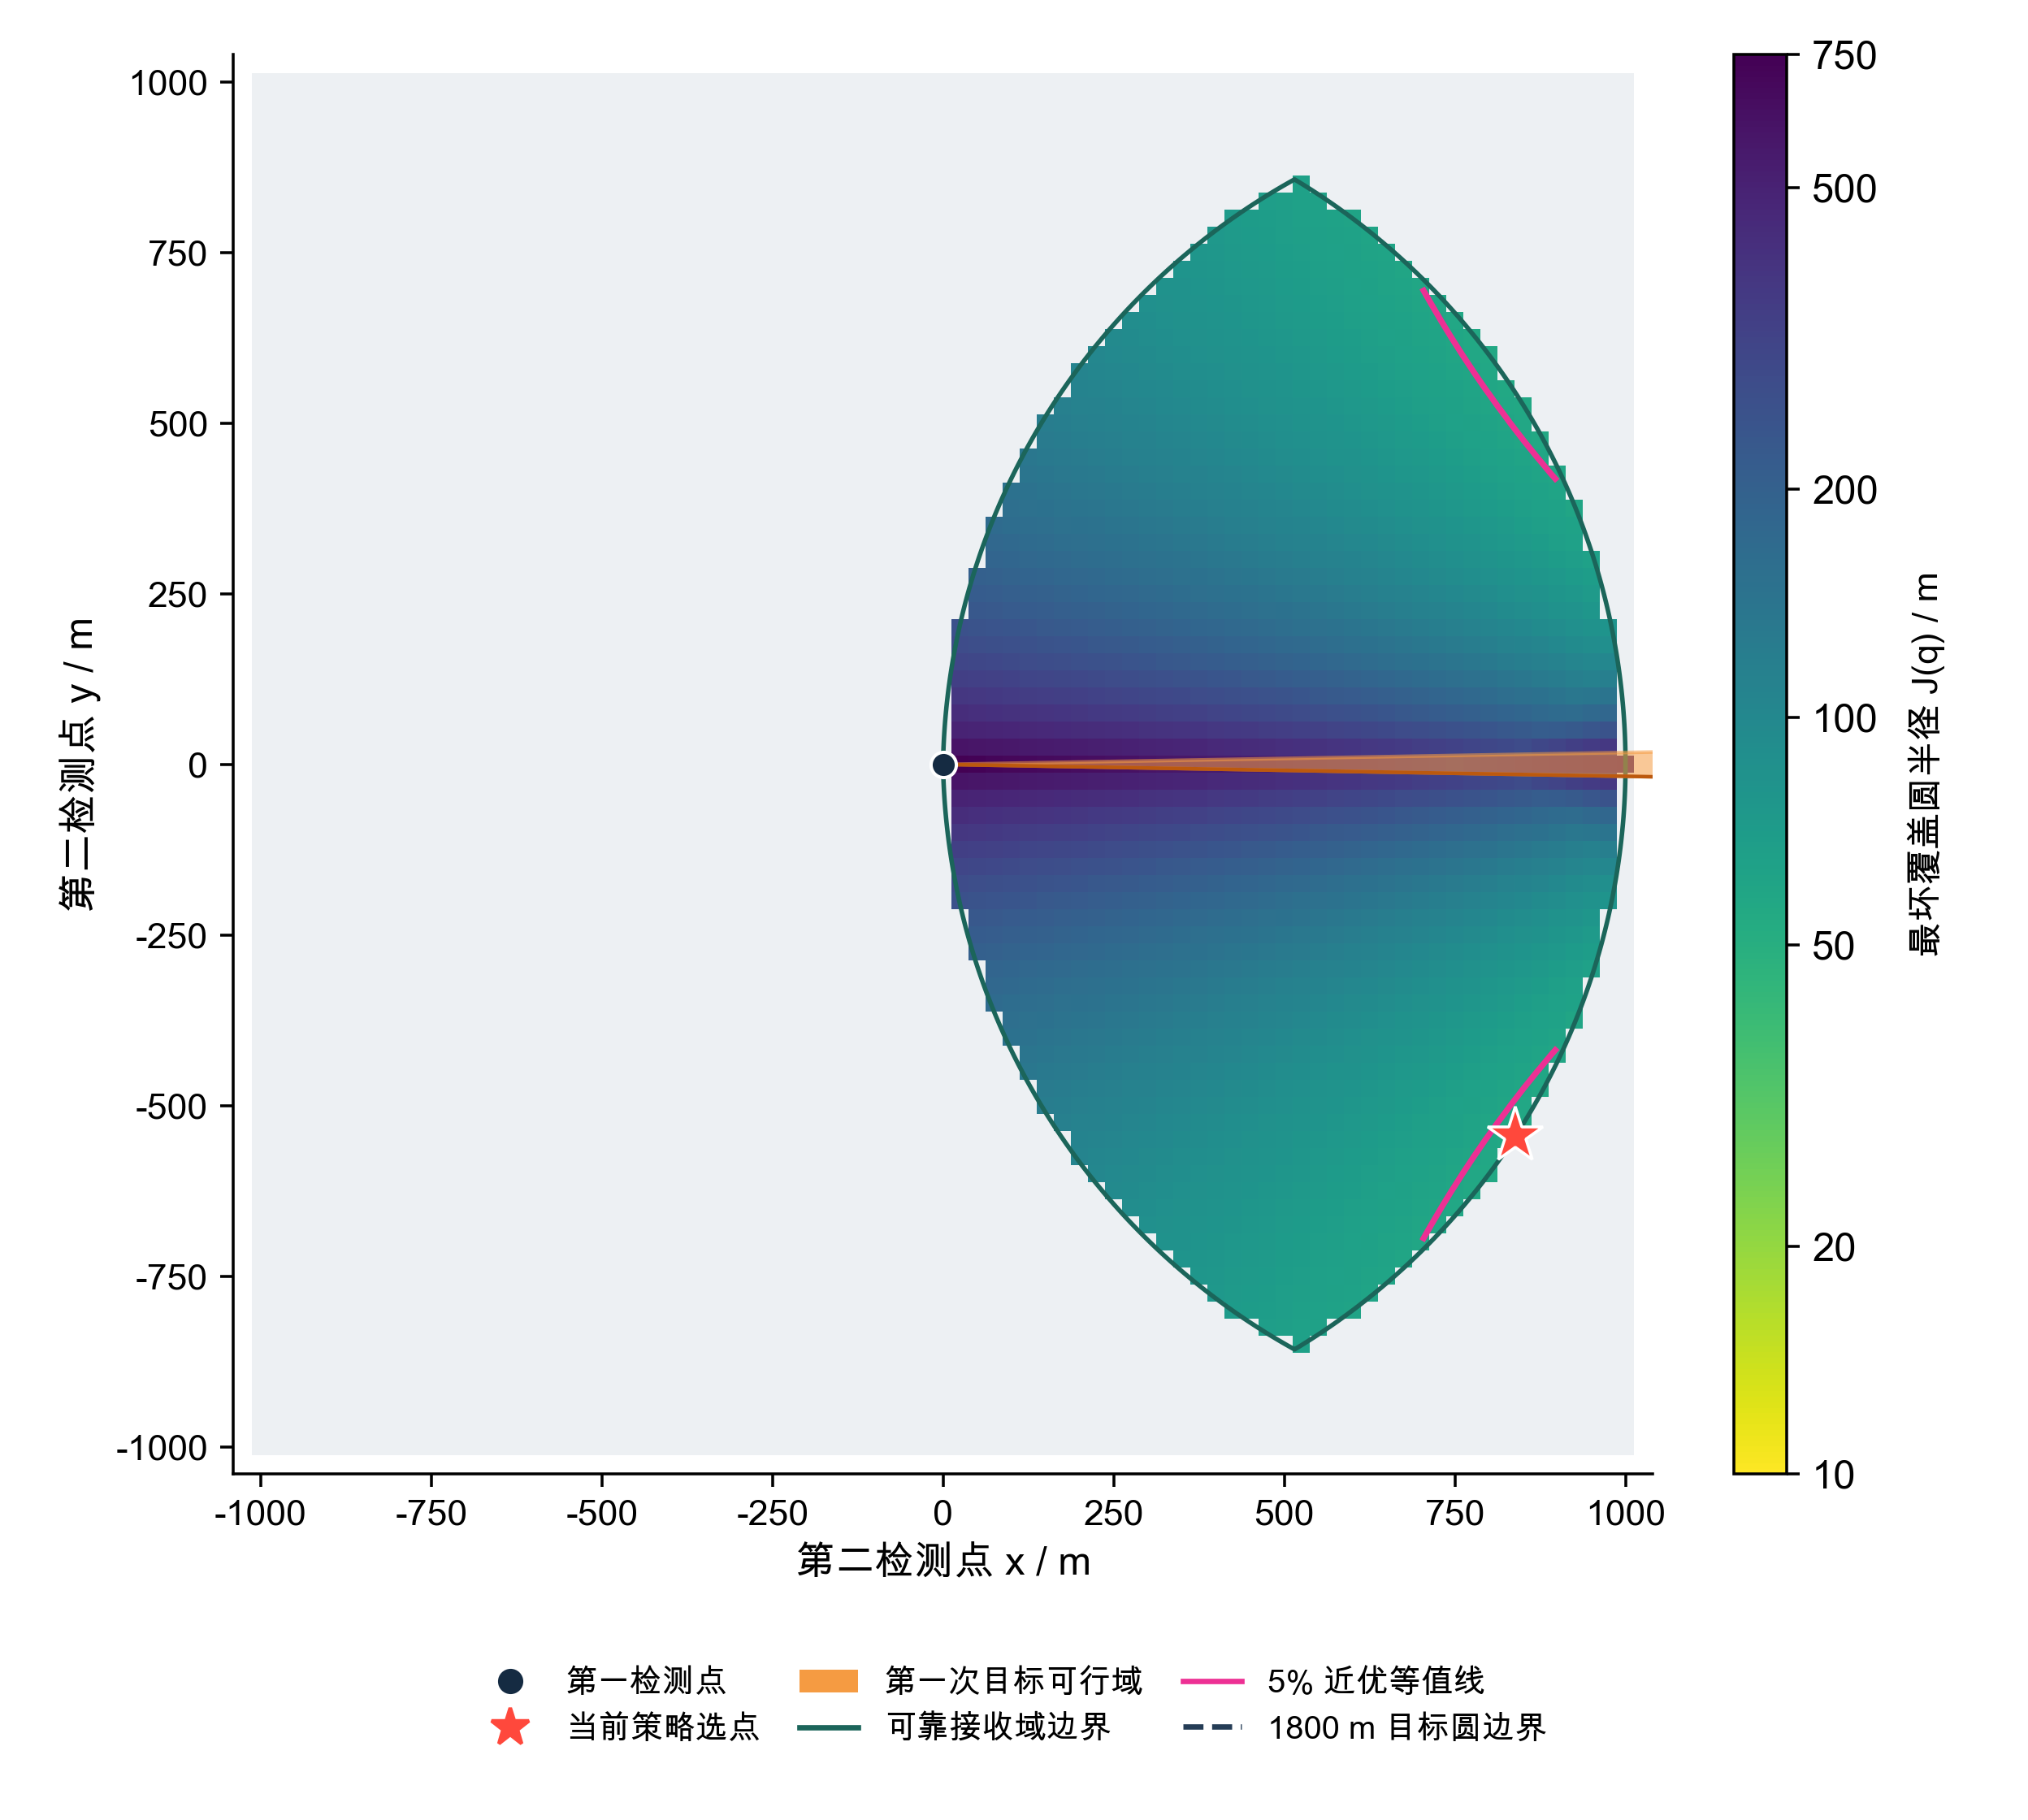
\includegraphics[width=\linewidth]{center_heatmap.png}
    \caption{第一检测点位于圆心，前向可行距离约为1500米。}
    \label{fig:q2-center}
  \end{subfigure}
  \hfill
  \begin{subfigure}[t]{0.48\textwidth}
    \centering
    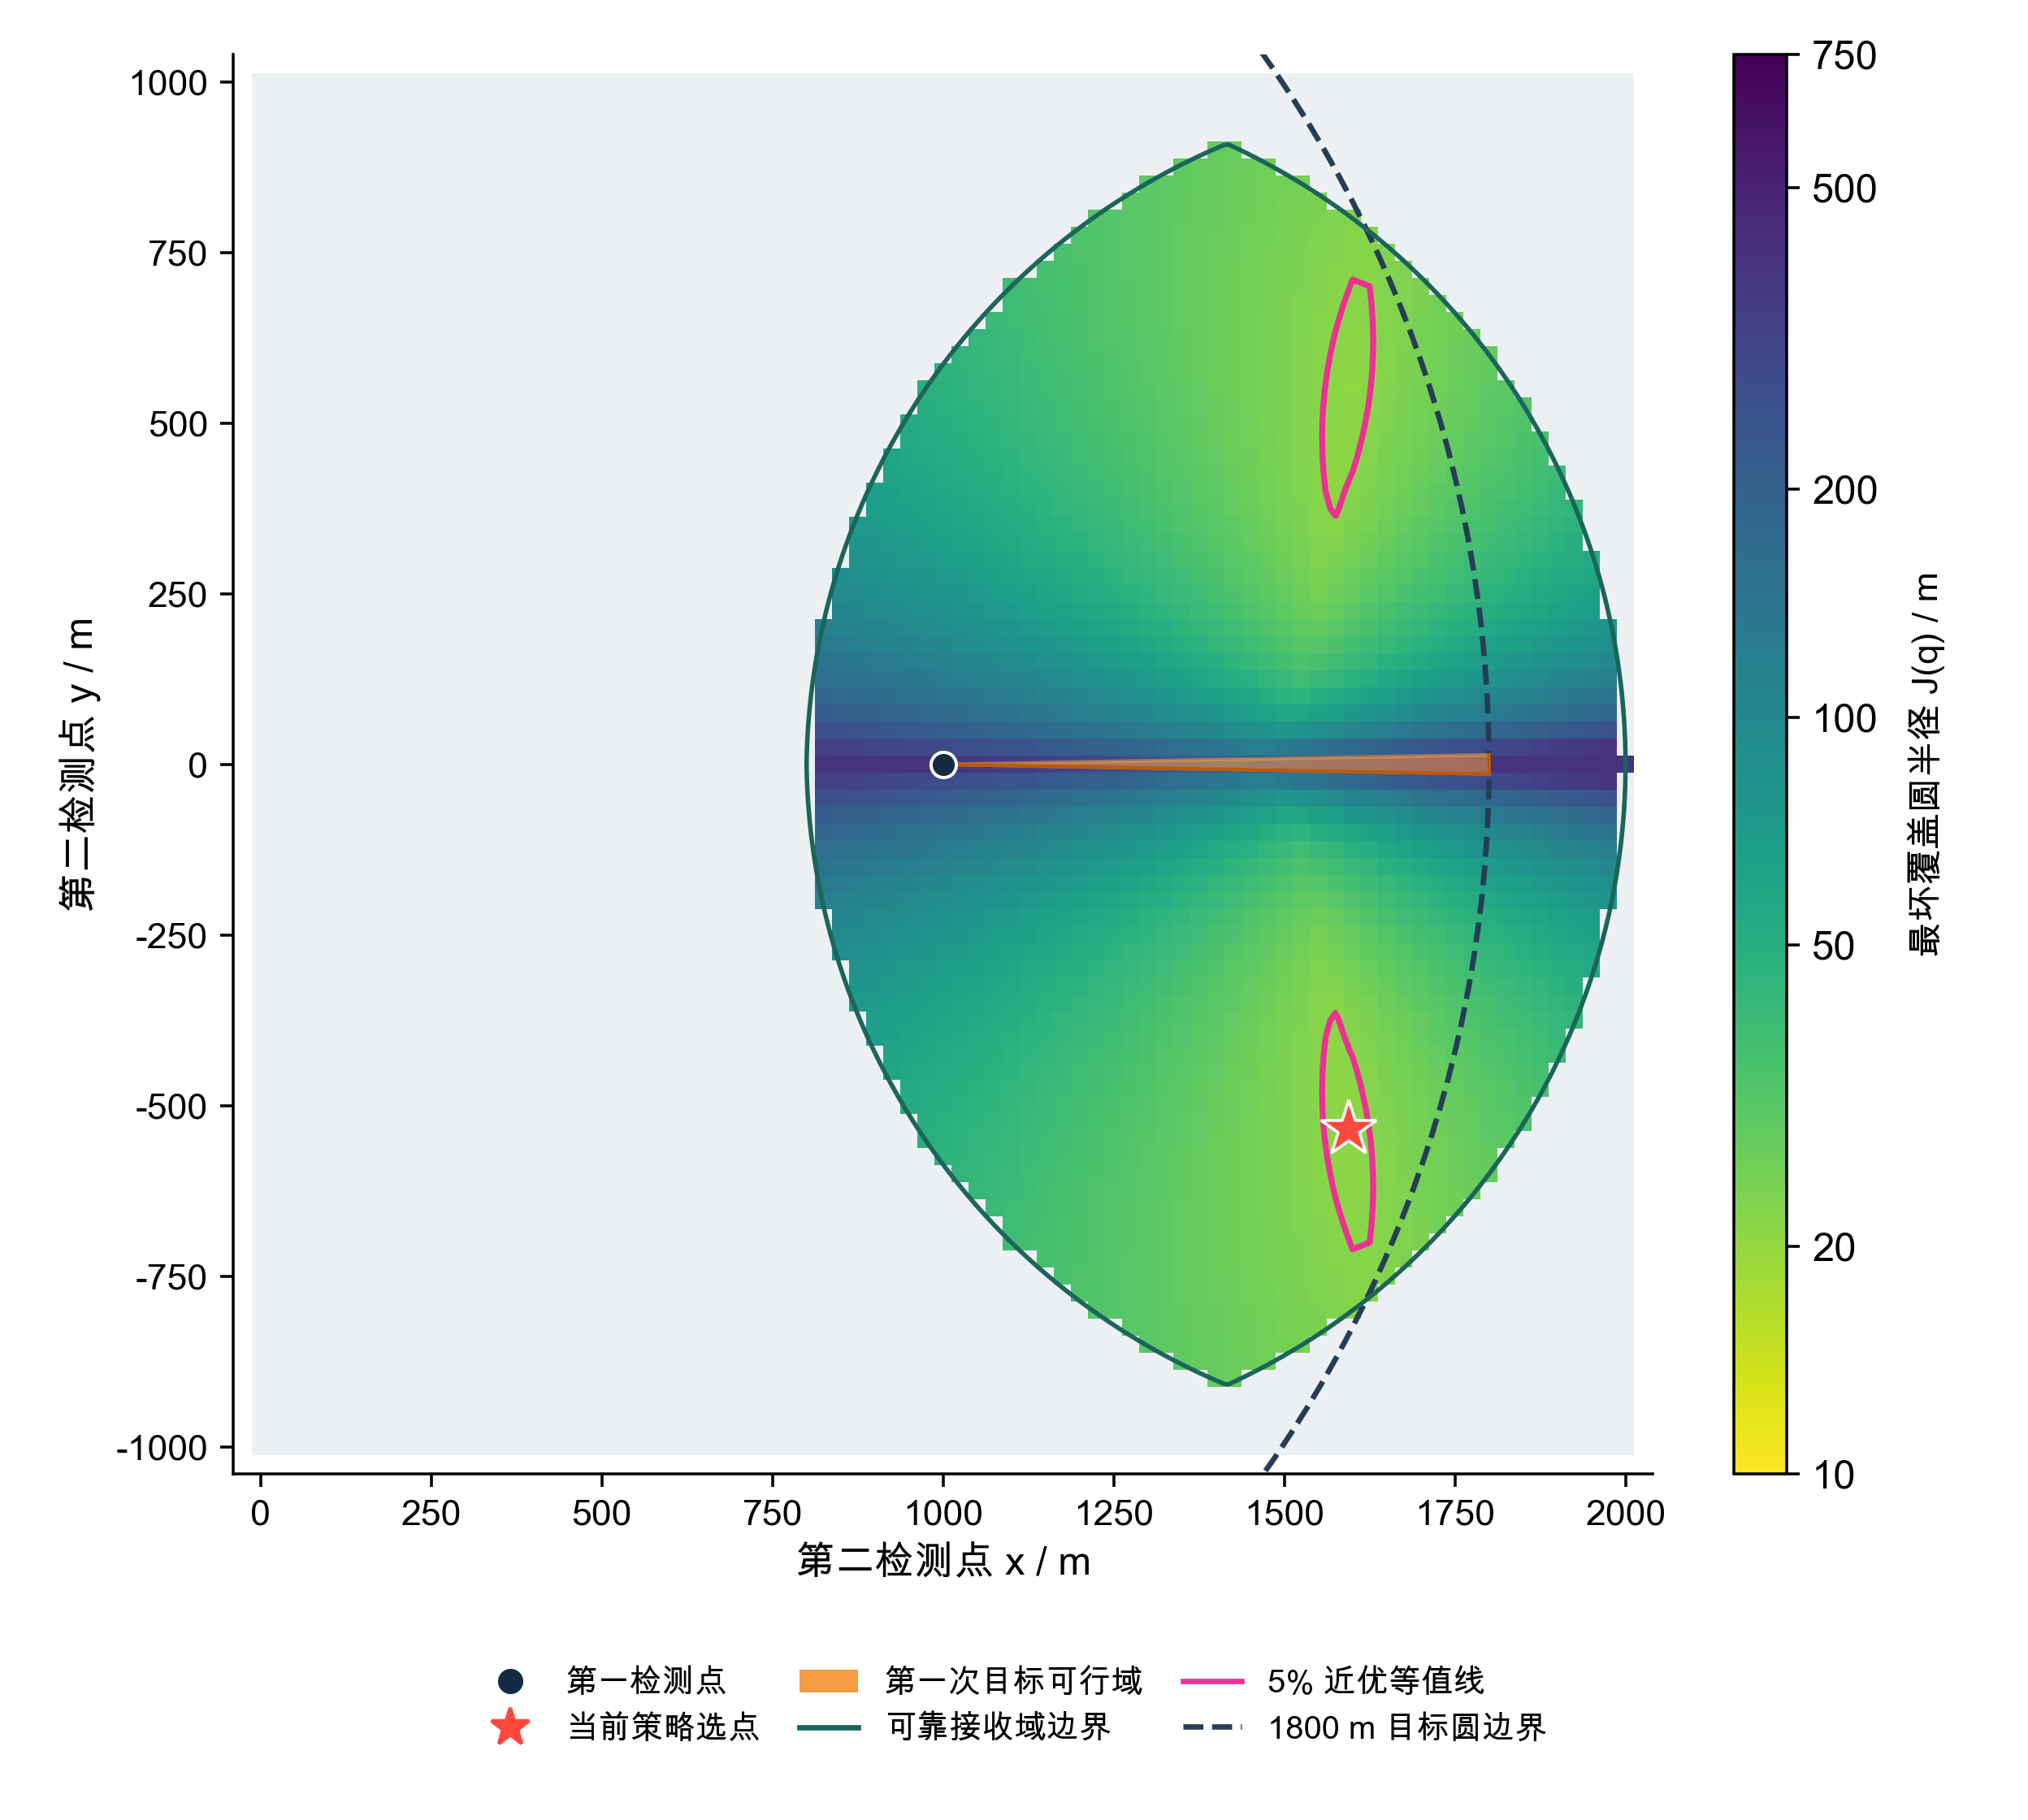
\includegraphics[width=\linewidth]{clipped_800m_heatmap.png}
    \caption{第一检测点为$(1000,0)$，前向可行距离被裁切至约800米。}
    \label{fig:q2-clipped}
  \end{subfigure}
  \caption{第二检测点候选区域的最坏覆盖圆半径热力图。两种情形的第一次示向度均为$0^\circ$，使用相同对数色标。红星表示当前策略输出，粉色等值线对应相对该策略值的5\%近优阈值。热力值采用25米网格逐点评分；圆域采用96边外接多边形，未来示向度按2度网格并补充关键角采样，接收约束角步长为0.05度。结果为数值近似，沿用忽略5米特殊返回的主模型。}
  \label{fig:q2-heatmaps}
\end{figure}

\FloatBarrier

由图~\ref{fig:q2-heatmaps}可见，第二检测点的选择由目标可行域的距离范围、
测向交会几何和可靠接收条件共同决定。沿第一次示向轴移动难以有效消除纵向位置
不确定性，因而较优检测点通常具有明显的横向位移。目标圆边界的裁切不仅缩短
目标可行域，还可能扩大可靠接收域，使策略能够以较短的移动距离形成有效交会。
在本文两个对称案例中，较优候选区域均呈上下镜像分布；当目标可行域的前向距离
由约 $1500\,\mathrm{m}$ 裁切至约 $800\,\mathrm{m}$ 时，当前策略的最坏覆盖半径
由 $55.84\,\mathrm{m}$ 降至 $20.59\,\mathrm{m}$。
